\documentclass[12pt,a4paper]{article}

% ─── Page Layout ───────────────────────────────────────────────────────────────
\usepackage[a4paper, margin=0.8in, headheight=14pt]{geometry}

% ─── Fonts (XeLaTeX) ───────────────────────────────────────────────────────────
\usepackage{fontspec}
\usepackage{unicode-math}
\setmainfont{TeX Gyre Pagella}
\setmonofont[Scale=0.88]{TeX Gyre Cursor}
\setmathfont{Latin Modern Math}

% ─── Packages ──────────────────────────────────────────────────────────────────
\usepackage{xcolor}
\usepackage{colortbl}
\usepackage{titlesec}
\usepackage{enumitem}
\usepackage{tabularx}
\usepackage{booktabs}
\usepackage{array}
\usepackage{amsmath}
\usepackage{tikz}
\usetikzlibrary{shapes.geometric, arrows.meta, positioning, calc, fit, decorations.pathreplacing}
\usepackage{tcolorbox}
\tcbuselibrary{skins, breakable}
\usepackage{hyperref}
\usepackage{fancyhdr}
\usepackage{graphicx}
\usepackage{microtype}
\hyphenpenalty=10000
\exhyphenpenalty=10000
\sloppy
\usepackage{caption}
\usepackage{setspace}
\usepackage{multirow}
\usepackage{tocloft}

% ─── Q&A helper ────────────────────────────────────────────────────────────────
\newcommand{\Q}[1]{\textbf{#1}\par\noindent\ignorespaces}

% ─── Colour Palette ────────────────────────────────────────────────────────────
\definecolor{myred}{RGB}{196,30,58}
\definecolor{mydark}{RGB}{30,30,50}
\definecolor{mygreen}{RGB}{14,120,80}
\definecolor{myteal}{RGB}{0,130,140}
\definecolor{myamber}{RGB}{180,100,0}
\definecolor{mypurple}{RGB}{100,30,160}
\definecolor{mygray}{RGB}{246,247,249}
\definecolor{mgframe}{RGB}{180,185,200}
\definecolor{watermark}{RGB}{145,150,170}
\definecolor{hdrred}{RGB}{250,232,235}
\definecolor{hdrgreen}{RGB}{220,244,233}
\definecolor{hdrteal}{RGB}{220,242,244}
\definecolor{hdramber}{RGB}{253,242,215}
\definecolor{hdrpurple}{RGB}{238,228,255}
\definecolor{hdrgray}{RGB}{238,240,245}
\definecolor{rowalt}{RGB}{250,251,253}

% ─── Section Formatting ────────────────────────────────────────────────────────
\titleformat{\section}
  {\large\bfseries\color{myred}}{\thesection.}{0.5em}{}
  [\vspace{1pt}{\color{myred}\rule{\linewidth}{0.8pt}}]
\titleformat{\subsection}
  {\normalsize\bfseries\color{myteal}}{\thesubsection}{0.5em}{}
\titlespacing*{\section}{0pt}{18pt}{7pt}
\titlespacing*{\subsection}{0pt}{11pt}{4pt}

% ─── Paragraph ─────────────────────────────────────────────────────────────────
\setlength{\parindent}{0pt}
\setlength{\parskip}{4pt}

% ─── TOC Styling ───────────────────────────────────────────────────────────────
\renewcommand{\cfttoctitlefont}{\large\bfseries\color{myred}}
\renewcommand{\cftaftertoctitle}{\par\noindent{\color{myred}\rule{\linewidth}{0.8pt}}}
\setlength{\cftbeforetoctitleskip}{0pt}
\setlength{\cftaftertoctitleskip}{6pt}
\renewcommand{\cftsecfont}{\normalsize\bfseries\color{mydark}}
\renewcommand{\cftsecpagefont}{\normalsize\bfseries\color{mydark}}
\renewcommand{\cftsecleader}{\cftdotfill{\cftdotsep}}
\setlength{\cftbeforesecskip}{7pt}
\renewcommand{\cftsubsecfont}{\small\color{mydark}}
\renewcommand{\cftsubsecpagefont}{\small\color{mydark}}
\setlength{\cftbeforesubsecskip}{3pt}
\setlength{\cftsubsecindent}{1.4em}

% ─── Table helpers ─────────────────────────────────────────────────────────────
\renewcommand{\arraystretch}{1.45}
\setlength{\tabcolsep}{6pt}
\arrayrulecolor{mydark}
\newcolumntype{B}[1]{>{\small\bfseries\raggedright\arraybackslash}m{#1}}
\newcolumntype{Y}{>{\small\raggedright\arraybackslash}X}
\renewcommand{\tabularxcolumn}[1]{m{#1}}

% ─── Header / Footer ───────────────────────────────────────────────────────────
\pagestyle{fancy}
\fancyhf{}
\fancyhead[L]{\small\color{myred}\textbf{PE-EC701A}\;\color{mydark}--- Microwave Theory and Technique}
\fancyhead[R]{\small\color{myteal}\textbf{Module 2 Notes}}
\fancyfoot[C]{\small\color{mydark}\thepage}
\fancyfoot[R]{\small\color{watermark}\textit{\copyright\ Biraj}}
\renewcommand{\headrulewidth}{0.5pt}
\renewcommand{\footrulewidth}{0.3pt}

% ─── Hyperref ──────────────────────────────────────────────────────────────────
\hypersetup{
  colorlinks=true, linkcolor=myteal, urlcolor=myteal,
  pdfauthor={Biraj Sarkar},
  pdftitle={PE-EC701A --- Module 2 Notes}
}

% ─── tcolorbox styles ──────────────────────────────────────────────────────────
\tcbset{
  tikzbox/.style={
    colback=mygray, colframe=mgframe, boxrule=0.6pt, arc=4pt,
    left=8pt, right=8pt, top=6pt, bottom=6pt,
    colbacktitle=mgframe, coltitle=mydark,
    fonttitle=\small\bfseries
  },
  defbox/.style={
    colback=hdrgreen, colframe=mygreen, boxrule=0.8pt, arc=4pt,
    left=9pt, right=9pt, top=6pt, bottom=6pt,
    colbacktitle=mygreen, coltitle=white,
    fonttitle=\small\bfseries
  },
  formulabox/.style={
    colback=hdrteal, colframe=myteal, boxrule=0.8pt, arc=4pt,
    left=9pt, right=9pt, top=7pt, bottom=7pt,
    colbacktitle=myteal, coltitle=white,
    fonttitle=\small\bfseries
  },
  examplebox/.style={
    colback=hdramber, colframe=myamber, boxrule=0.8pt, arc=4pt,
    left=9pt, right=9pt, top=6pt, bottom=6pt,
    colbacktitle=myamber, coltitle=white,
    fonttitle=\small\bfseries
  },
  masonbox/.style={
    colback=hdrpurple, colframe=mypurple, boxrule=0.8pt, arc=4pt,
    left=9pt, right=9pt, top=6pt, bottom=6pt,
    colbacktitle=mypurple, coltitle=white,
    fonttitle=\small\bfseries
  },
  exambox/.style={
    colback=hdrpurple, colframe=mypurple, boxrule=1pt, arc=5pt,
    left=10pt, right=10pt, top=8pt, bottom=8pt,
    colbacktitle=mypurple, coltitle=white,
    fonttitle=\bfseries,
    breakable, title after break={\textbf{Frequently Asked / Viva Questions (contd.)}}}
}
% Make all boxes breakable across pages
\tcbset{breakable}

% ─── TikZ styles ───────────────────────────────────────────────────────────────
\tikzset{
  block/.style={rectangle, draw=myteal, fill=hdrteal,
    text width=2.4cm, align=center, minimum height=0.95cm,
    font=\small, rounded corners=3pt, line width=0.7pt},
  redblock/.style={rectangle, draw=myred, fill=hdrred,
    text width=2.4cm, align=center, minimum height=0.95cm,
    font=\small, rounded corners=3pt, line width=0.7pt},
  netnode/.style={rectangle, draw=myteal, fill=hdrteal,
    text width=1.5cm, align=center, minimum height=0.8cm,
    font=\small, rounded corners=3pt, line width=0.7pt},
  sumjunc/.style={circle, draw=myamber, fill=hdramber,
    minimum size=0.62cm, font=\small, line width=0.8pt},
  snode/.style={circle, draw=mypurple, fill=hdrpurple,
    minimum size=0.55cm, font=\footnotesize, line width=0.7pt},
  arrow/.style={-Stealth, thick, color=mydark},
  redarrow/.style={-Stealth, thick, color=myred},
  line/.style={thick, color=mydark}
}

% ═══════════════════════════════════════════════════════════════════════════════
\begin{document}
% ═══════════════════════════════════════════════════════════════════════════════

\begin{center}
  {\LARGE\bfseries\color{myred} PE-EC701A --- Microwave Theory and Technique}\\[5pt]
  {\normalsize\color{mydark} Semester VII \quad$\bullet$\quad 3L:0T:0P \quad$\bullet$\quad 3 Credits}\\[3pt]
  {\normalsize\color{myteal}\textbf{Module 2 Exam Notes: Mathematical Model of Microwave Transmission}}\\[3pt]
  {\small\color{mydark} CGEC \;$|$\; B.Tech ECE (2023--27) \;$|$\; \textit{Biraj Sarkar}}
\end{center}
\vspace{2pt}
\noindent{\color{myred}\rule{\linewidth}{1.5pt}}
\vspace{2pt}

\hypersetup{linkcolor=mydark}
\tableofcontents
\hypersetup{linkcolor=myteal}
\newpage

% ===============================================================================
\section{Concept of Wave Modes}
% ===============================================================================

When electromagnetic waves propagate along a guide structure, the boundaries dictate how the fields are oriented. These field distributions are classified as modes.

\begin{tcolorbox}[defbox]
\textbf{Wave Mode:} A specific configuration of electric and magnetic fields that satisfies Maxwell's equations and the boundary conditions of the transmission structure. Modes are characterized by their cutoff frequencies and spatial patterns.
\end{tcolorbox}

\subsection{Classification of Modes}
We classify electromagnetic modes based on the presence of longitudinal field components along the direction of propagation (assumed to be the $z$-axis):
\begin{itemize}[leftmargin=*, itemsep=3pt]
  \item \textbf{TEM (Transverse Electromagnetic) Mode:}
    Both the electric and magnetic fields are entirely transverse to the direction of propagation.
    \begin{equation}
      E_z = 0 \quad \text{and} \quad H_z = 0
    \end{equation}
  \item \textbf{TE (Transverse Electric) Mode:}
    The electric field is completely transverse to the direction of propagation, while the magnetic field has a longitudinal component.
    \begin{equation}
      E_z = 0 \quad \text{and} \quad H_z \ne 0
    \end{equation}
  \item \textbf{TM (Transverse Magnetic) Mode:}
    The magnetic field is completely transverse to the direction of propagation, while the electric field has a longitudinal component.
    \begin{equation}
      H_z = 0 \quad \text{and} \quad E_z \ne 0
    \end{equation}
  \item \textbf{Hybrid Modes (HE/EH):}
    Both electric and magnetic fields have non-zero longitudinal components.
    \begin{equation}
      E_z \ne 0 \quad \text{and} \quad H_z \ne 0
    \end{equation}
\end{itemize}

\subsection{Field Lines in Waveguide Cross-Sections}
The physical layout of the electric ($\vec{E}$) and magnetic ($\vec{H}$) fields is visualized below:

\begin{tcolorbox}[tikzbox, title={Field Distribution in Coaxial (TEM) and Rectangular Waveguide ($\text{TE}_{10}$)}]
\centering
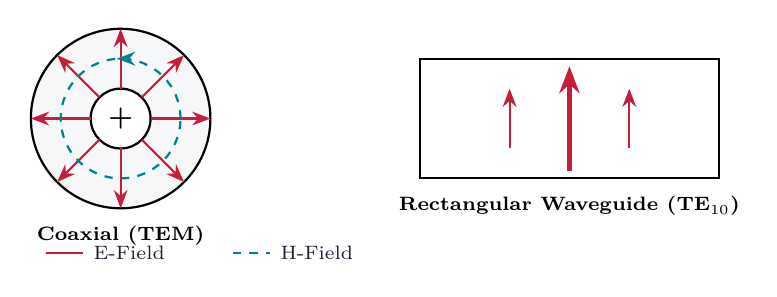
\begin{tikzpicture}[scale=0.95]
  % Coaxial (TEM)
  \draw[thick, fill=mygray] (-3,0) circle (1.2cm);
  \draw[thick, fill=white] (-3,0) circle (0.4cm);
  \node[font=\bfseries] at (-3,0) {+};
  \node[below, font=\scriptsize\bfseries] at (-3,-1.3) {Coaxial (TEM)};
  
  % Radial E-field lines
  \foreach \angle in {0, 45, 90, 135, 180, 225, 270, 315} {
    \draw[-Stealth, color=myred, thick] (-3,0) +(\angle:0.4) -- +(\angle:1.2);
  }
  % Concentric H-field lines
  \draw[dashed, color=myteal, thick] (-3,0) circle (0.8cm);
  \draw[-Stealth, color=myteal, thick] (-3,0.8) -- (-3.05,0.8);
  
  % Rectangular Waveguide (TE10)
  \draw[thick] (1,-0.8) rectangle (5,0.8);
  \node[below, font=\scriptsize\bfseries] at (3,-0.9) {Rectangular Waveguide ($\text{TE}_{10}$)};
  
  % E-field vertical lines (sinusoidal profile in center)
  \draw[-Stealth, color=myred, thick] (2.2,-0.4) -- (2.2,0.4);
  \draw[-Stealth, color=myred, line width=1.5pt] (3.0,-0.7) -- (3.0,0.7);
  \draw[-Stealth, color=myred, thick] (3.8,-0.4) -- (3.8,0.4);
  
  % H-field closed loops (represented in cross section as points/crosses or loops)
  % Show E-field legend
  \draw[thick, color=myred] (-4,-1.8) -- (-3.5,-1.8) node[right, font=\scriptsize, color=mydark] {E-Field};
  \draw[dashed, thick, color=myteal] (-1.5,-1.8) -- (-1.0,-1.8) node[right, font=\scriptsize, color=mydark] {H-Field};
\end{tikzpicture}
\end{tcolorbox}

% ===============================================================================
\section{Proof of Non-Existence of TEM Mode in Hollow Waveguides}
% ===============================================================================

A central mathematical model shows that TEM waves cannot propagate inside single-conductor hollow waveguides.

\begin{tcolorbox}[defbox, title={\textbf{Theorem}}]
TEM waves cannot exist inside a hollow waveguide formed by a single closed conductor. They require at least two distinct conductors (e.g., coaxial line) to propagate.
\end{tcolorbox}

\subsubsection{Mathematical Proof}
Assume a TEM wave propagates along the $z$-direction in a hollow waveguide with a single conductor wall $C$. For a TEM mode, by definition:
\begin{equation*}
  E_z = 0 \quad \text{and} \quad H_z = 0
\end{equation*}
From Maxwell's curl equation for the electric field:
\begin{equation*}
  \nabla \times \vec{E} = -j\omega\mu \vec{H}
\end{equation*}
Analyzing the $z$-component of the curl:
\begin{equation}
  \frac{\partial E_y}{\partial x} - \frac{\partial E_x}{\partial y} = -j\omega\mu H_z
\end{equation}
Since $H_z = 0$, this yields:
\begin{equation}
  \frac{\partial E_y}{\partial x} - \frac{\partial E_x}{\partial y} = 0
\end{equation}
This indicates that the transverse electric field $\vec{E}_t = E_x \hat{a}_x + E_y \hat{a}_y$ has a curl of zero in the transverse plane. Therefore, the transverse electric field can be expressed as the gradient of a scalar electrostatic potential function $\Phi(x, y)$:
\begin{equation}
  \vec{E}_t = -\nabla_t \Phi(x, y)
\end{equation}
Next, we invoke Gauss's Law in the charge-free dielectric region inside the waveguide:
\begin{equation*}
  \nabla \cdot \vec{E} = 0 \implies \frac{\partial E_x}{\partial x} + \frac{\partial E_y}{\partial y} + \frac{\partial E_z}{\partial z} = 0
\end{equation*}
Since $E_z = 0$, the divergence equation reduces to the transverse plane:
\begin{equation}
  \nabla_t \cdot \vec{E}_t = 0
\end{equation}
Substituting $\vec{E}_t = -\nabla_t \Phi$ into the divergence equation yields:
\begin{equation}
  \nabla_t^2 \Phi(x, y) = 0 \quad (\text{Laplace's Equation})
\end{equation}
Now we apply the boundary conditions on the waveguide boundary $C$. Since the wall is a Perfect Electric Conductor (PEC), the tangential electric field must vanish on $C$.
This implies the conductor boundary is an equipotential surface:
\begin{equation}
  \Phi(x, y) = \Phi_0 \quad (\text{constant}) \quad \text{on boundary } C
\end{equation}
According to the \textbf{uniqueness theorem} of Laplace's equation:
If a potential $\Phi$ satisfies Laplace's equation ($\nabla^2 \Phi = 0$) within a closed region bounded by a single conductor at a constant potential $\Phi_0$, then the potential must be constant everywhere inside that region:
\begin{equation}
  \Phi(x, y) = \Phi_0 \quad \text{for all } x, y \text{ inside } C
\end{equation}
Taking the gradient of a constant potential to find the electric field:
\begin{equation}
  \vec{E}_t = -\nabla_t \Phi_0 = 0
\end{equation}
If the electric field is zero everywhere inside the waveguide, then by Maxwell's equations, the magnetic field is also zero:
\begin{equation}
  \vec{H}_t = 0
\end{equation}
Thus, no electromagnetic fields can exist inside the guide. Therefore, \textbf{TEM modes cannot exist inside a hollow, single-conductor waveguide} (Q.E.D.).

% ===============================================================================
\section{Losses Associated with Microwave Transmission}
% ===============================================================================

Energy propagating down a microwave line attenuates due to three primary physical loss mechanisms:

\subsection{Conductor Losses (Skin Effect)}
At microwave frequencies, current does not distribute uniformly across the conductor cross-section but crowds near the surface.
\begin{tcolorbox}[defbox]
\textbf{Skin Depth ($\delta$):} The depth into a conductor at which the electromagnetic wave amplitude decays to $1/e$ (approx. $36.8\%$) of its surface value.
\end{tcolorbox}

\begin{tcolorbox}[formulabox, title={\textbf{Skin Depth and Surface Resistance}}]
The skin depth $\delta$ is given by:
\begin{equation}
  \delta = \frac{1}{\sqrt{\pi f \mu \sigma}} \quad (\text{m})
\end{equation}
The corresponding surface resistance $R_s$ is:
\begin{equation}
  R_s = \frac{1}{\sigma \delta} = \sqrt{\frac{\pi f \mu}{\sigma}} \quad (\Omega/\text{square})
\end{equation}
Where:
\begin{itemize}[leftmargin=1.5em, itemsep=1pt, topsep=2pt]
  \item[] $f$ = frequency of operation (Hz)
  \item[] $\mu$ = permeability of the conductor ($\text{H/m}$)
  \item[] $\sigma$ = conductivity of the metal ($\text{S/m}$)
\end{itemize}
\end{tcolorbox}

\subsection{Dielectric Losses}
Dielectric losses occur in the medium filling the waveguide due to the rotation of polar molecules under high-frequency alternating electric fields. It is quantified using the loss tangent ($\tan \delta$):
\begin{equation}
  \alpha_d = \frac{\omega \epsilon''}{2 \beta} \approx \frac{\pi \sqrt{\epsilon_r} \tan \delta}{\lambda_0} \quad (\text{Np/m})
\end{equation}

\subsection{Radiation Losses}
Radiation losses occur primarily in open-boundary lines (e.g., Microstrip lines) where fields are not completely enclosed, allowing some energy to radiate outward as radio waves.

% ===============================================================================
\section{Concept of Wave Impedance}
% ===============================================================================

\begin{tcolorbox}[defbox]
\textbf{Wave Impedance ($Z_w$):} The ratio of the transverse electric field to the transverse magnetic field for a propagating mode. It represents the characteristic resistance that the wave encounters as it travels.
\end{tcolorbox}

The wave impedance depends heavily on the mode type (TE or TM) and the operating frequency:

\begin{tcolorbox}[formulabox, title={\textbf{Wave Impedance Formulations}}]
Let $\eta = \sqrt{\mu/\epsilon}$ be the intrinsic impedance of the dielectric medium. The wave impedances for TE and TM modes are:
\begin{align}
  Z_{\text{TE}} &= \frac{\eta}{\sqrt{1 - \left(\frac{f_c}{f}\right)^{\!2}}} \quad (\Omega) \\
  Z_{\text{TM}} &= \eta \sqrt{1 - \left(\frac{f_c}{f}\right)^{\!2}} \quad (\Omega)
\end{align}
Where:
\begin{itemize}[leftmargin=1.5em, itemsep=1pt, topsep=2pt]
  \item[] $f_c$ = Cutoff frequency of the specific mode
  \item[] $f$ = Operating frequency
\end{itemize}
\textbf{Critical Limits:}
\begin{itemize}[leftmargin=1.5em, itemsep=1pt]
  \item For $f < f_c$ (below cutoff): Impedance is purely imaginary, indicating evanescent (non-propagating) fields.
  \item For $f \to \infty$: Both $Z_{\text{TE}}$ and $Z_{\text{TM}}$ approach the intrinsic impedance $\eta$ of the medium.
\end{itemize}
\end{tcolorbox}

% ===============================================================================
% MANDATORY QUICK REVISION PAGE
% ===============================================================================
\newpage
\begin{center}
  {\large\bfseries\color{myred} Quick Revision --- Module II}\\[3pt]
  {\small\color{mydark} Mathematical Model of Microwave Transmission $|$ PE-EC701A}
\end{center}
\noindent{\color{myred}\rule{\linewidth}{1.2pt}}
\vspace{4pt}

\begin{tcolorbox}[formulabox, title={\textbf{Key Formulas at a Glance}}]
\renewcommand{\arraystretch}{1.3}
\begin{tabularx}{\linewidth}{B{4.5cm} X}
Skin Depth              & $\delta = \frac{1}{\sqrt{\pi f \mu \sigma}}$ \\[4pt]
Surface Resistance      & $R_s = \sqrt{\frac{\pi f \mu}{\sigma}}$ \\[4pt]
TE Wave Impedance       & $Z_{\text{TE}} = \frac{\eta}{\sqrt{1 - (f_c/f)^2}}$ \\[4pt]
TM Wave Impedance       & $Z_{\text{TM}} = \eta \sqrt{1 - (f_c/f)^2}$ \\[4pt]
Intrinsic Impedance     & $\eta = \sqrt{\frac{\mu}{\epsilon}} \approx 377\,\Omega$ (in free space)
\end{tabularx}
\end{tcolorbox}

\begin{tcolorbox}[defbox, title={\textbf{One-Line Definitions}}]
\begin{itemize}[leftmargin=*, itemsep=2.5pt, topsep=0pt]
  \item \textbf{Wave Mode:} A valid mathematical field pattern satisfying boundary conditions.
  \item \textbf{TEM Mode:} A mode with zero electric and magnetic fields in the direction of propagation.
  \item \textbf{Wave Impedance:} The ratio of transverse electric field to transverse magnetic field.
  \item \textbf{Skin Depth:} The distance in a metal where current density drops to $36.8\%$ of surface value.
  \item \textbf{Uniqueness Theorem:} Electrostatic theorem proving Laplace's solution is unique under boundary limits.
  \item \textbf{Evanescent Wave:} An attenuated wave that does not carry real power, occurring below cutoff.
  \item \textbf{Loss Tangent:} A measure of energy dissipation in a lossy dielectric material.
\end{itemize}
\end{tcolorbox}

\begin{tcolorbox}[exambox, title={\textbf{Frequently Asked / Viva Questions}}]
\begin{enumerate}[topsep=0pt, label=\textbf{Q\arabic*.}, itemsep=5pt]
  \item \Q{Why can TEM waves not exist inside a hollow waveguide?}
    Because the waveguide wall is a single conductor that acts as an equipotential boundary. Inside, Laplace's equation forces the potential to be constant, making the electric fields zero.
  \item \Q{What transmission structures support TEM waves?}
    Structures with two or more isolated conductors, such as coaxial lines, striplines, and microstrip lines.
  \item \Q{How does skin depth vary with frequency?}
    It is inversely proportional to the square root of frequency ($\delta \propto 1/\sqrt{f}$). Higher frequencies yield thinner skin depths.
  \item \Q{Why do conductor losses increase at microwave frequencies?}
    Because current is confined to a very thin layer (skin depth), effectively reducing the cross-sectional area of conduction and increasing resistance.
  \item \Q{Explain the behaviour of $Z_{\text{TE}}$ as frequency approaches the cutoff frequency $f_c$ from above.}
    As $f \to f_c^+$, the denominator $\sqrt{1-(f_c/f)^2} \to 0$, causing the wave impedance $Z_{\text{TE}}$ to approach infinity.
  \item \Q{What happens to the wave impedance of a TM mode below cutoff ($f < f_c$)?}
    The term inside the radical becomes negative, making the wave impedance purely reactive/imaginary, indicating no real power propagation.
  \item \Q{What is the physical significance of the loss tangent ($\tan \delta$)?}
    It represents the ratio of the lossy conduction current density to the lossless displacement current density in a dielectric.
  \item \Q{Why do we use copper or silver plating inside microwave guides?}
    To reduce conductor losses. Since currents flow within a few microns of the surface, a thin layer of highly conductive material reduces surface resistance $R_s$.
  \item \Q{State the intrinsic impedance of free space.}
    $\eta_0 = \sqrt{\mu_0/\epsilon_0} \approx 120\pi \approx 377\,\Omega$.
  \item \Q{What is the difference between TE and TM modes?}
    In TE modes, the longitudinal electric field is zero ($E_z = 0, H_z \ne 0$). In TM modes, the longitudinal magnetic field is zero ($H_z = 0, E_z \ne 0$).
  \item \Q{How does the cutoff frequency affect mode propagation?}
    Waves only propagate if their operating frequency exceeds the cutoff frequency ($f > f_c$). Below cutoff, waves decay exponentially.
  \item \Q{What are hybrid modes?}
    Modes where both the longitudinal electric and magnetic fields are non-zero ($E_z \ne 0$ and $H_z \ne 0$). They are common in optical fibers.
\end{enumerate}
\tcbset{colbacktitle=mgframe, coltitle=mydark}
\end{tcolorbox}

\begin{tcolorbox}[tikzbox, title={Comparison of Wave Propagation Modes}]
\renewcommand{\arraystretch}{1.4}
\par\noindent
\begin{tabularx}{\linewidth}{|B{3.2cm}|Y|Y|Y|}
\hline
\rowcolor{hdrgray}
\textbf{Feature} & \textbf{TEM Mode} & \textbf{TE Mode} & \textbf{TM Mode} \\
\hline
\textbf{Longitudinal $E_z$} & $E_z = 0$ & $E_z = 0$ & $E_z \ne 0$ \\
\hline
\rowcolor{rowalt}
\textbf{Longitudinal $H_z$} & $H_z = 0$ & $H_z \ne 0$ & $H_z = 0$ \\
\hline
\textbf{Hollow Guide?} & No & Yes & Yes \\
\hline
\rowcolor{rowalt}
\textbf{Wave Impedance} & $Z_w = \eta$ & $Z_w = \eta / \sqrt{1-(f_c/f)^2}$ & $Z_w = \eta \sqrt{1-(f_c/f)^2}$ \\
\hline
\textbf{Cutoff Freq $f_c$} & $f_c = 0$ & $f_c > 0$ & $f_c > 0$ \\
\hline
\end{tabularx}
\end{tcolorbox}

\end{document}
